\clearpage
\makeatletter
\efloat@restorefloats
\makeatother


\begin{appendix}
\section{}
\setlength{\parindent}{0.0in}
\setlength{\leftskip}{0.0in}

\hypertarget{the-mathematical-development-of-the-f-test-w-test-and-f-test-numerical-example}{%
\subsection{\texorpdfstring{The Mathematical Development of the
\emph{F}-test, \emph{W}-test, and \emph{F}*-test: Numerical
Example}{The Mathematical Development of the F-test, W-test, and F*-test: Numerical Example}}\label{the-mathematical-development-of-the-f-test-w-test-and-f-test-numerical-example}}

A summary is presented in Table A1. The complete example is available on
Github. The DV is a score that can vary from 0 to 40. The IV is a
three-level factor A (levels = \(A_1\), \(A_2\) and \(A_3\)).

\begin{figure}
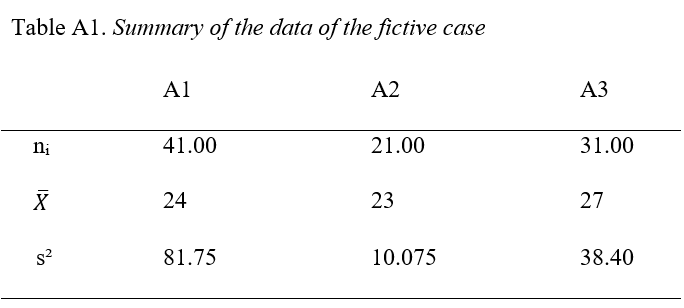
\includegraphics[width=1\linewidth]{Rmarkdown folder/Rmarkdown inputs/TableA1} \end{figure}

The global mean (i.e.~the mean of the global dataset) is a weighted mean
of the group means:

\[\frac{(41*24)+(21*23)+(31*27)}{41+21+31}=\frac{2304}{93} \approx 24.77\]

The \emph{F}-test statistic and degrees of freedom are computed by
applying formulas (1), (2) and (3):

\[
F=\frac{\frac{1}{3-1}[41*(24-\frac{2304}{93})^2+21*(23-\frac{2304}{93})^2+31*(27-\frac{2304}{93})^2]}
{\frac{1}{93-3}[(41-1)*81.75+(21-1)*10.07+(31-1)*38.40]} \approx 2.38
\]

\[
df_n=3-1=2
\]

\[
df_d=93-3=90
\]

The \emph{F}*-test and his degrees of freedom are computed by applying
formulas 4, 5 and 6:

\[
F^*=\frac{41*(24-\frac{2304}{93})^2+21*(23-\frac{2304}{93})^2+31*(27-\frac{2304}{93})^2}{(1-\frac{41}{93})*81.75+(1-\frac{21}{93})*10.07+(1-\frac{31}{93})*38.40} \approx 3.09
\]

\[
df_n=3-1=2
\]

\[
df_d=\frac{1}{\frac{(\frac{(1-\frac{41}{93})*81.75}{\sum_{j=1}^k(1-\frac{n_j}{N})s_j^2})^2}{41-1}+\frac{(\frac{(1-\frac{21}{93})*10.07}{\sum_{j=1}^k(1-\frac{n_j}{N})s_j^2})^2}{21-1}+\frac{(\frac{(1-\frac{31}{93})*38.40}{\sum_{j=1}^k(1-\frac{n_j}{N})s_j^2})^2}{31-1}} \approx 81.15
\]

\[ Where \sum_{j=1}^k(1-\frac{n_j}{N})*s_j^2 \approx 79.11\]

Finally, the \emph{W}-test and his degrees of freedom are computed in
applying formulas 7, 8 and 9:

\[
W=\frac{\frac{1}{3-1}[\frac{41}{81.75}(24-\bar{X'})^2+\frac{21}{10.07}(23-\bar{X'})^2+\frac{31}{38.40}(27-\bar{X'})^2]}
{\frac{2(3-2)}{3^2-1}[(\frac{1}{41-1})(1-\frac{\frac{41}{81.75}}{w})^2+(\frac{1}{21-1})(1-\frac{\frac{21}{10.07}}{w})^2+(\frac{1}{31-1})(1-\frac{\frac{31}{38.40}}{w})^2]+1} \approx 4.61
\]

Where:

\(w=\sum_{j=1}^k w_j \approx 3.39\)

\(\bar{X'}=\frac{\sum_{j=1}^k (w_j\bar{x_j})}{w} \approx 24.10\)

\[
df_n=3-1
\]

\[
df_d=\frac{3^2-1}{3[\frac{(1-\frac{w_j}{w})^2}{41-1}+\frac{(1-\frac{w_j}{w})^2}{21-1}+\frac{(1-\frac{w_j}{w})^2}{31-1}]} \approx 59.32
\]

One should notice that in this example, the biggest sample size has the
biggest variance. As previously mentioned, it means that the
\emph{F}-test will be too conservative, because the \emph{F} value
decreases. The \emph{F}*-test will also be a little too conservative,
even if the test is less affected than the \emph{F}-test. As a
consequence: \emph{W} \textgreater{} \emph{F}* \textgreater{} \emph{F}.
\end{appendix}
